\subsection{System Design}\label{subsection:B}

The system consists of essential components, including a Jetson Orin Nano and/or Raspberry Pi to process deep learning models. The Drone-Kit API and MAVLink protocol facilitate communication with the Cube Black flight controller, which ultimately controls the drone's motor and navigation. The system flow chart is depicted in Fig.~\ref{fig2b1}.

Two embedded devices, the Jetson Nano and Raspberry Pi, are incorporated into the drone to compare their performance. Additionally, a SIK radio block is utilized to send the drone's status back to a Laptop/PC for real-time monitoring. For added safety, a Flysky FS-i6 6CH 2.4GHz RC Transmitter and iA6B Receiver are included to enable manual drone control.

    \begin{figure}[H]
        \centerline{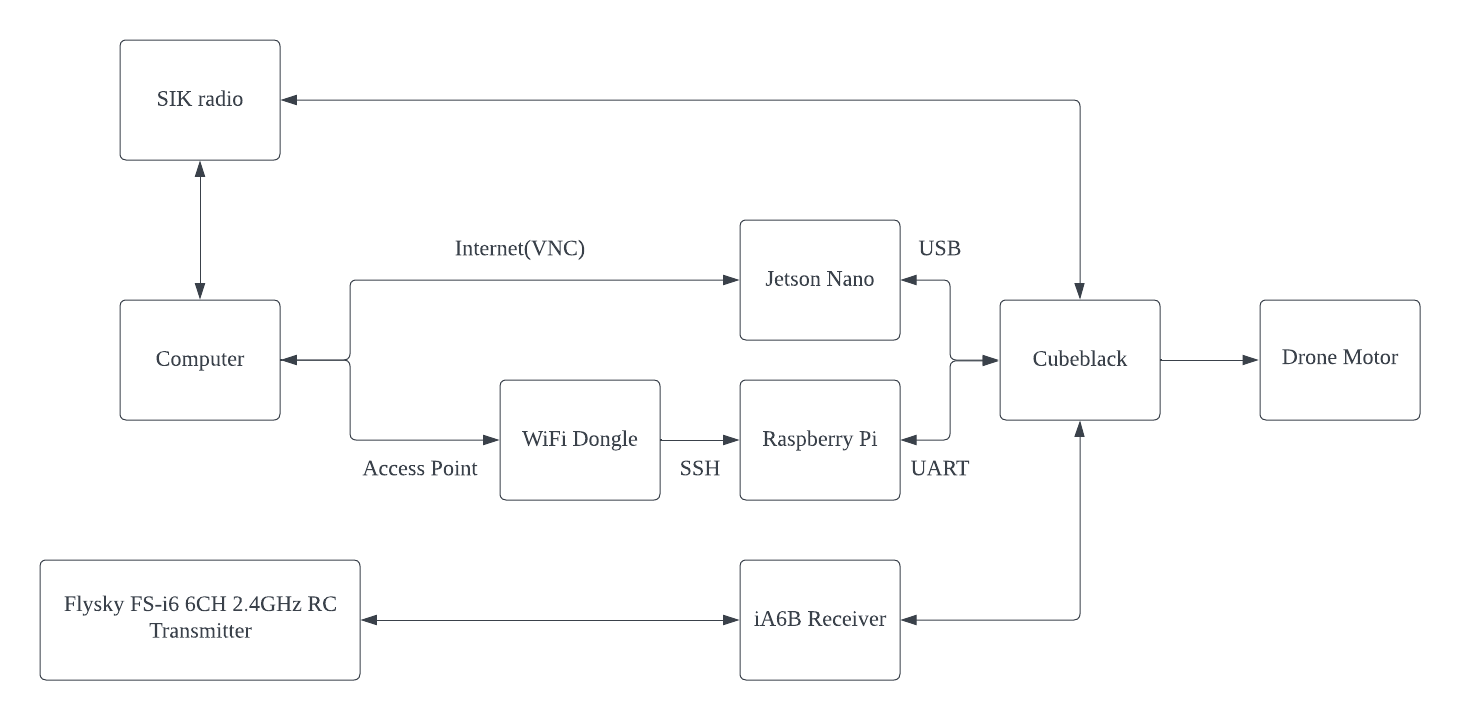
\includegraphics[width=0.5\textwidth]{Figures/Methods/System Flow Chart.png}}
        \caption{System Flow Chart.}
        \label{fig2b1}
    \end{figure}

    \begin{figure}[H]
        \centerline{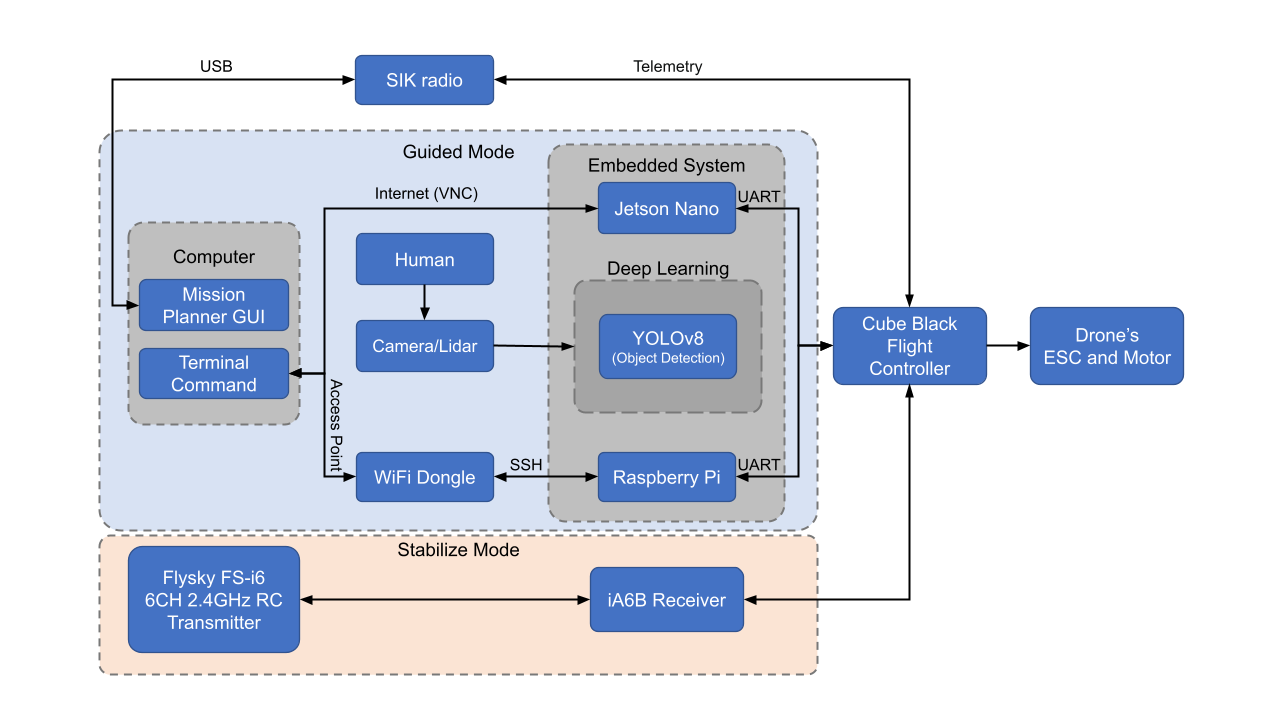
\includegraphics[width=0.5\textwidth]{Figures/Methods/System_Overall_Design.png}}
        \caption{Overall System Design.}
        \label{fig2b2}
    \end{figure}

Fig.~\ref{fig2b2} provides a detailed overview of the system design. The process starts with capturing an image of people using a camera. The image is then analyzed using Deep Learning's YOLOv8 object detection model, which runs on the Embedded System Jetson Orin Nano and/or Raspberry Pi. YOLOv8 is used to detect human in the image (Please note sections \ref{subsection:C} below for more information on YOLOv8), while LiDAR scans for the distance between the human and the drone. (Please note sections \ref{subsection:D} below for more information on LiDAR)


For manual control, we use the Flysky FS-i6 6CH 2.4GHz RC Transmitter in Stabilize Mode, which disables pre-arming checking and puts the drone in an unstable mode. However, to operate the drone using scripts, it must be set to Guided Mode, which allows pre-arming checks to ensure the drone is in a safe condition to complete the pollination task.